\chapter{Diversiteit van eencellige organismen}\label{ch:b2:unicellular-diversity}

Een druppel slootwater onder de microscoop bevat een groene cel die met
twee flagellen roeit, een pantoffelvormige ciliaat die bacteriën naar
haar celmond veegt, een glazig kiezelwier dat over het objectglaasje
glijdt en, te klein om goed te zien, duizend bacteriën. Elk daarvan is
één cel en elk is een volledig organisme: het voedt zich, beweegt,
neemt waar, groeit, plant zich voort en sterft als één enkele cel. Het
grootste deel van de levende wereld is altijd zo geweest. Dit
hoofdstuk behandelt het eencellige organisme als een ontwerpprobleem
--- wat één cel wel en niet kan --- en overziet de antwoorden die
prokaryoten en eukaryoten hebben gevonden, tot het punt waarop cellen
bij elkaar beginnen te blijven.

\section{Eén cel, alle functies}

\begin{definition}[Eencellig, koloniaal, meercellig]\label{def:b2:unicellular-diversity:unicellular}
Een organisme is \emph{eencellig}\index{eencellig organisme} wanneer
één cel alle levensfuncties uitvoert --- voeding, uitwisseling,
beweging, voortplanting --- en op zichzelf leeft. Het is
\emph{koloniaal}\index{koloniaal organisme} wanneer cellen van één
soort na de deling aan elkaar blijven zitten, maar elk ervan, eenmaal
losgemaakt, op zichzelf kan blijven leven. Het is
\emph{meercellig}\index{meercellig organisme} wanneer zijn cellen van
verschillende typen zijn, van elkaar afhangen en slechts enkele ervan
(de kiembaan) nakomelingen achterlaten. Tot de eencellige organismen
behoren alle archaea, bijna alle bacteriën en de meeste lijnen van
eukaryoten; de informele naam \emph{\omterm{def:b2:unicellular-diversity:protist}{protist}} dekt de eencellige
eukaryoten, die niet één groep vormen maar vele.
\end{definition}

\begin{example}[Zes bewoners van een druppel]\label{ex:b2:unicellular-diversity:drop}
\emph{Escherichia coli}, een staafje van \qty{2}{\micro m} lang,
zwemt met een bundel flagellen en deelt zich om de twintig minuten
als het gevoed wordt. \emph{Chlamydomonas}, een groene alg van
\qty{10}{\micro m} doorsnede, roeit met twee flagellen naar het licht
dat ze met een oogvlek waarneemt. \emph{Paramecium}, een ciliaat van
\qty{200}{\micro m}, is bedekt met duizenden trilharen, voedt zich via
een celmond en hoost water naar buiten met twee \omterm{prop:b2:unicellular-diversity:osmoregulation}{contractiele
vacuolen}. Een kiezelwier leeft in een tweedelige schaal van
kiezelzuur, versierd met poriën. \emph{Amoeba} vloeit voort door
schijnvoetjes uit te steken en omsluit wat ze tegenkomt. Een gistcel
laat aan haar zijkant een dochtercel uitknoppen. Zes antwoorden, van
sterk uiteenlopende grootte en machinerie, op één probleem.
\end{example}

\begin{omfigure}
\begin{tikzpicture}[x=1.9cm]
  % log scale from 0.1 um to 100 mm : position = log10(size in um) + 1
  \draw[thick] (0,0) -- (6,0);
  \foreach \p/\l in {0/{\qty{0.1}{\micro m}},1/{\qty{1}{\micro m}},2/{\qty{10}{\micro m}},3/{\qty{100}{\micro m}},4/{\qty{1}{mm}},5/{\qty{10}{mm}},6/{\qty{100}{mm}}}
    \draw (\p,0.12) -- (\p,-0.12) node[below, font=\scriptsize] {\l};
  \foreach \p/\c/\l in {0.5/omDef/mycoplasma, 1.3/omDef/{\emph{E.~coli}}, 1.7/omDef/gist, 2.0/omProp/{\emph{Chlamydomonas}}, 2.7/omProp/kiezelwieren, 3.3/omProp/{\emph{Paramecium}}, 3.65/omProp/{\emph{Amoeba proteus}}, 3.9/omThm/{\emph{Thiomargarita} (een bacterie)}, 5.7/omProp/{\emph{Acetabularia}}}
    { \fill[\c] (\p,0) circle (0.05); \node[rotate=60, anchor=west, font=\scriptsize, \c, inner sep=1pt] at (\p,0.12) {\l}; }
  \node[font=\scriptsize, anchor=north] at (3,-0.55) {celgrootte (logaritmische schaal)};
\end{tikzpicture}

{\small De grootte van eencellige organismen beslaat vijf ordes van
grootte. Prokaryoten (blauw) liggen rond een micrometer; eukaryote
cellen (oranje) zijn tien tot honderd keer groter; de grootste
afzonderlijke cellen --- een reuzenzwavelbacterie, de alg
\emph{Acetabularia} --- zijn uitzonderingen die de tekst verklaart.}
\end{omfigure}

\begin{proposition}[Oppervlak, volume en de grens aan de grootte]\label{prop:b2:unicellular-diversity:surface}
\index{oppervlakte-volumeverhouding}
Een cel wisselt uit met haar omgeving via haar oppervlak en verbruikt
naar verhouding van haar volume. Voor een bol met straal $r$ is de
\emph{\omterm{prop:b2:unicellular-diversity:surface}{oppervlakte-volumeverhouding}}
\[
\frac{S}{V} = \frac{4\pi r^2}{\tfrac{4}{3}\pi r^3} = \frac{3}{r},
\]
zodat een verdubbeling van de straal het beschikbare oppervlak per
eenheid cytoplasma halveert. Een cel die voor de bevoorrading van haar
inwendige op diffusie door haar membraan steunt, kan dus niet
onbeperkt groeien: bij een zekere straal voldoet de aanvoer door het
oppervlak niet meer aan de vraag van het volume. Dezelfde wet verklaart
waarom kleine cellen per gram metabool het actiefst zijn, en waarom
grote cellen afgeplat, langgerekt, gevacuoliseerd of vol inwendige
membranen zijn.
\end{proposition}

\begin{theorem}[Tijd om een afstand te diffunderen]\label{thm:b2:unicellular-diversity:diffusion}
\index{diffusietijd}
Een molecuul met diffusiecoëfficiënt $D$ zwerft in willekeurige
stappen rond; na een tijd $t$ is zijn gemiddelde kwadratische
verplaatsing langs één as $\langle x^2\rangle = 2Dt$. De tijd die
nodig is om door diffusie alleen een afstand $x$ af te leggen, is dus
\[
t \approx \frac{x^2}{2D},
\]
die groeit met het \emph{kwadraat} van de afstand. Met
$D \approx \qty{1e-9}{m^2/s}$ voor een klein molecuul in water duurt
het oversteken van een bacterie (\qty{1}{\micro m}) een halve
milliseconde; het oversteken van een cel van \qty{1}{mm} zou acht
minuten duren, en van een meter zestien jaar.
\end{theorem}
\begin{proof}
Laat het molecuul stappen met lengte $\ell$ zetten, willekeurig naar
links of naar rechts, telkens na $\tau$ seconden. Na $n$ stappen is zijn
verplaatsing $x = \sum_i \varepsilon_i \ell$ met $\varepsilon_i = \pm 1$
onafhankelijk, dus $\langle x\rangle = 0$ en $\langle x^2\rangle =
\sum_i \langle\varepsilon_i^2\rangle \ell^2 = n\ell^2$ (de
kruistermen middelen uit tot nul). Met $n = t/\tau$ is dit $\langle x^2\rangle
= (\ell^2/\tau)\,t$, en met $D = \ell^2/2\tau$ volgt
$\langle x^2\rangle = 2Dt$. Stelt men $\langle x^2\rangle = x^2$, dan
volgt de tijd.
\end{proof}

\begin{theorem}[Diffusieve aanvoer naar een bolvormige cel]\label{thm:b2:unicellular-diversity:supply}
\index{diffusiebegrensde opname}
Een bolvormige cel met straal $r_0$ die elk molecuul van een opgeloste
stof dat haar oppervlak bereikt opneemt, in een medium waar de
concentratie ver weg $c_\infty$ bedraagt, ontvangt in de stationaire
toestand een flux (moleculen per seconde) van
\[
J = 4\pi D r_0\, c_\infty .
\]
De aanvoer groeit slechts met $r_0$, de vraag met
$r_0^3$: voorbij een zekere straal verhongert een cel die door diffusie wordt gevoed.
\end{theorem}
\begin{proof}
In de stationaire toestand is het aantal moleculen dat per seconde
een bol met straal $r > r_0$ passeert voor elke bol hetzelfde, $J = 4\pi r^2 D\,
(\mathrm{d}c/\mathrm{d}r)$ (de wet van Fick, met de flux naar binnen
gericht). Dus is $r^2\,\mathrm{d}c/\mathrm{d}r = J/4\pi D$ constant;
integreren van $r_0$, waar $c = 0$, tot oneindig, waar $c = c_\infty$, geeft
$c_\infty = (J/4\pi D)\int_{r_0}^{\infty} r^{-2}\,\mathrm{d}r =
J/(4\pi D r_0)$, waaruit $J = 4\pi D r_0 c_\infty$.
\end{proof}

\begin{example}[Hoe groot kan een door diffusie gevoede cel zijn?]\label{ex:b2:unicellular-diversity:howbig}
Een aerobe cel verbruikt zuurstof met ongeveer $q = \qty{0.02}{mol/m^3/s}$
cytoplasma (een stevig tempo). Haar vraag is $q \cdot \tfrac{4}{3}\pi
r_0^3$; de aanvoer uit met lucht verzadigd water ($c_\infty =
\qty{0.25}{mol/m^3}$, $D = \qty{2e-9}{m^2/s}$) is $4\pi D r_0
c_\infty$. Gelijkstellen geeft $r_0^2 = 3Dc_\infty/q = 3\times 2\times 10^{-9}
\times 0.25/0.02 = \qty{7.5e-8}{m^2}$, dus $r_0 \approx
\qty{270}{\micro m}$. Echte actieve cellen blijven hier ruim onder,
omdat zuurstof ook \emph{in} de cel moet diffunderen; de zwavelbacterie
\emph{Thiomargarita} van \qty{750}{\micro m} omzeilt de grens door
vrijwel geheel uit een vacuole te bestaan, met een cytoplasma dat
slechts een dunne schil van enkele micrometers vormt.
\end{example}

\begin{omfigure}
\begin{tikzpicture}
\begin{axis}[
  width=0.8\linewidth, height=6.2cm,
  axis x line=bottom, axis y line=left,
  xmode=log, ymode=log,
  xmin=0.3, xmax=1000, ymin=1e-6, ymax=1e4,
  xlabel={celstraal (\unit{\micro m})}, ylabel={moleculen per seconde (relatief)},
  xlabel style={font=\small, at={(axis description cs:0.5,-0.1)}, anchor=north},
  ylabel style={font=\small},
  tick label style={font=\small},
  legend style={font=\small, at={(0.03,0.97)}, anchor=north west, draw=none},
  clip=false,
]
\addplot[very thick, omDef, domain=0.3:1000, samples=40] {x/10};
\addlegendentry{aanvoer door diffusie, $\propto r$}
\addplot[very thick, omThm, domain=0.3:1000, samples=40] {(x/10)^3/1000*1.0};
\addlegendentry{vraag van het cytoplasma, $\propto r^3$}
\draw[dashed, gray] (axis cs:270,1e-6) -- (axis cs:270,27);
\node[font=\scriptsize, anchor=west] at (axis cs:300,3e-4) {hongerstraal};
\end{axis}
\end{tikzpicture}

{\small De aanvoer door het oppervlak groeit met $r$, de vraag met
$r^3$ (logaritmische assen). Waar de lijnen elkaar snijden, kan een
cel die alleen door diffusie wordt gevoed haar inwendige niet langer
bevoorraden; voor een actieve aerobe cel ligt dat snijpunt bij enkele
honderden micrometers.}
\end{omfigure}

\section{Diversiteit van de prokaryoten}

\begin{definition}[De prokaryote cel]\label{def:b2:unicellular-diversity:prokaryote}
Een \emph{prokaryoot}\index{prokaryoot} (de bacteriën en de archaea,
twee domeinen die evenveel van elkaar verschillen als elk van beide
van ons) is een cel zonder kern of door een membraan omgeven
organellen: één circulair chromosoom in een \emph{nucleoïde}\index{nucleoïde},
vaak met kleine extra ringen die \emph{plasmiden}\index{plasmide}
heten, ribosomen vrij in een cytoplasma van \qtyrange{0.5}{2}{\micro m},
een plasmamembraan dat de ademhalings- of fotosyntheseketens draagt,
en een stevige \emph{celwand}\index{celwand!bacteriële} die weerstand
biedt aan de turgor van een cytoplasma dat enkele bar boven zijn
omgeving staat. Er zijn weinig vormen, en ze hebben een naam:
\emph{coccus} (bol), \emph{bacil} (staaf), \emph{spirillum} en
\emph{spirocheet} (schroeven), \emph{vibrio} (komma); cellen kunnen
na de deling in paren, ketens, tetraden of trossen bijeen blijven.
\end{definition}

\begin{proposition}[Twee omhulsels: grampositief en gramnegatief]\label{prop:b2:unicellular-diversity:gram}
\index{gramkleuring}\index{peptidoglycaan}
De bacteriële wand is opgebouwd uit \emph{peptidoglycaan}, ketens van
twee afwisselende suikers die door korte peptiden tot één reusachtig
molecuul rond de cel zijn verknoopt. \emph{Grampositieve} bacteriën
hebben een dikke laag (\qtyrange{20}{80}{nm}) buiten één enkel
membraan en houden de kristalviolette kleurstof van de gramkleuring
vast; \emph{gramnegatieve} bacteriën hebben een dunne laag (enkele
nanometers) ingeklemd tussen het plasmamembraan en een \emph{buitenmembraan}
waarvan het buitenste blad uit lipopolysacharide bestaat, en ze
verliezen de kleurstof. Het buitenmembraan, doorboord door porines,
is een tweede barrière: het houdt veel antibiotica en detergentia
tegen, en daarom zijn infecties met gramnegatieve bacteriën moeilijker
te behandelen. Archaea hebben noch peptidoglycaan noch de
esterlipiden van alle andere cellen: hun membranen bestaan uit
ethergebonden isoprenoïdketens, die soms als monolaag de hele dubbellaag
overspannen, wat ze stabiel houdt in kokend zuur.
\end{proposition}

\begin{omfigure}
\begin{tikzpicture}[scale=0.9, every node/.style={font=\scriptsize}]
  % Gram-positive
  \begin{scope}
    \fill[omDef!15] (0,0) rectangle (4,1.6);
    \node at (2,0.4) {cytoplasma};
    \fill[omDef!60] (0,1.6) rectangle (4,1.85);
    \node[right] at (4.05,1.72) {plasmamembraan};
    \fill[omProp!50] (0,1.85) rectangle (4,3.0);
    \foreach \y in {2.0,2.25,...,2.85} \draw[omProp!90!black] (0.1,\y) -- (3.9,\y);
    \node[right, align=left] at (4.05,2.45) {dik peptidoglycaan\\(\qtyrange{20}{80}{nm})};
    \node[above, font=\small\bfseries] at (2,3.05) {grampositief};
  \end{scope}
  % Gram-negative
  \begin{scope}[xshift=7.6cm]
    \fill[omDef!15] (0,0) rectangle (4,1.6);
    \node at (2,0.4) {cytoplasma};
    \fill[omDef!60] (0,1.6) rectangle (4,1.85);
    \node[right] at (4.05,1.72) {plasmamembraan};
    \fill[omProp!50] (0,2.05) rectangle (4,2.25);
    \draw[omProp!90!black] (0.1,2.15) -- (3.9,2.15);
    \node[right] at (4.05,2.15) {dun peptidoglycaan};
    \node at (2,1.95) {periplasma};
    \fill[omThm!50] (0,2.55) rectangle (4,2.85);
    \foreach \x in {0.6,2.0,3.4} \fill[white] (\x-0.12,2.55) rectangle (\x+0.12,2.85);
    \node[right] at (4.05,2.7) {buitenmembraan met porines};
    \foreach \x in {0.2,0.5,...,3.9} \draw[omThm!80!black, thick] (\x,2.85) -- (\x,3.1);
    \node[right] at (4.05,3.15) {lipopolysacharide};
    \node[above, font=\small\bfseries] at (2,3.3) {gramnegatief};
  \end{scope}
\end{tikzpicture}

{\small De twee bacteriële omhulsels in doorsnede. Links: één membraan
onder een dikke laag peptidoglycaan. Rechts: een dunne laag
peptidoglycaan in het periplasma tussen twee membranen, waarvan het
buitenste bezet is met porines en bedekt met lipopolysacharide.}
\end{omfigure}

\begin{proposition}[De bacteriële flagel en chemotaxis]\label{prop:b2:unicellular-diversity:flagellum}
\index{flagel!bacteriële}\index{chemotaxis}
De bacteriële \emph{flagel} is een stijf schroefvormig filament van het
eiwit flagelline, \qty{20}{nm} dik en enkele lichaamslengten lang, dat
wordt rondgedraaid door een rotatiemotor in het omhulsel. De motor
wordt niet door ATP aangedreven, maar door protonen die langs de
elektrochemische gradiënt over het membraan stromen, zo'n \num{1000}
protonen per omwenteling bij tot \num{300} omwentelingen per seconde.
Bij \emph{E.~coli} bundelen de flagellen zich wanneer ze allemaal
tegen de klok in draaien en duwen ze de cel in een rechte \emph{run}
vooruit; keert er één of meer om, dan valt de bundel uiteen en
\emph{tuimelt} de cel naar een nieuwe, willekeurige richting.
\emph{Chemotaxis} is de sturing van deze willekeurige wandeling: de
cel meet of de concentratie van een lokstof in de laatste seconde is
gestegen en onderdrukt in dat geval het tuimelen. Ze stuurt door het
heden met het recente verleden te vergelijken --- langs haar baan ---
omdat over haar eigen lengte van \qty{1}{\micro m} geen gradiënt
meetbaar is.
\end{proposition}
\begin{proof}[Bewijsmateriaal]
Berg en Brown (1972) volgden afzonderlijke cellen van \emph{E.~coli} in
drie dimensies met een volgmicroscoop: runs van ongeveer een seconde
bij \qty{20}{\micro m/s}, tuimelingen van een tiende seconde, en in
een gradiënt van serine waren de runs die de gradiënt op gingen
langer, terwijl de runs die hem af gingen niet korter werden. Een cel
die met één flagel aan een objectglaasje werd vastgezet, liet haar
hele lichaam ronddraaien, wat bewees dat de motor roteert; cellen
waarvan de motor van de ATP-synthese was ontkoppeld, zwommen nog zolang
er een protongradiënt kon worden opgelegd, wat de brandstof aanwees.
\end{proof}

\begin{omfigure}
\begin{tikzpicture}[every node/.style={font=\scriptsize}]
  % run and tumble path without gradient
  \begin{scope}
    \draw[very thick, omDef] (0,0) -- (1.2,0.5) -- (0.7,1.4) -- (1.9,1.8) -- (2.6,0.9) -- (3.4,1.5) -- (3.0,2.5);
    \foreach \p in {(1.2,0.5),(0.7,1.4),(1.9,1.8),(2.6,0.9),(3.4,1.5)} \fill[omThm] \p circle (0.06);
    \node[align=center] at (1.8,-0.5) {geen gradiënt:\\runs van gelijke lengte, willekeurige wendingen};
  \end{scope}
  \begin{scope}[xshift=6cm]
    \shade[left color=white, right color=omExo!50] (-0.3,-0.2) rectangle (5.2,3.0);
    \draw[very thick, omDef] (0,0.3) -- (0.9,0.8) -- (0.6,1.3) -- (2.4,1.5) -- (2.2,2.2) -- (4.6,2.4);
    \foreach \p in {(0.9,0.8),(0.6,1.3),(2.4,1.5),(2.2,2.2)} \fill[omThm] \p circle (0.06);
    \node[align=center] at (2.4,-0.5) {lokstof neemt naar rechts toe:\\runs de gradiënt op duren langer};
    \node[anchor=south east] at (5.1,2.6) {meer lokstof};
  \end{scope}
\end{tikzpicture}

{\small Run en tuimeling. Links: zonder gradiënt voert de cel een
willekeurige wandeling uit, waarbij elke run (blauw) eindigt met een
tuimeling (rode stip). Rechts: wanneer een lokstof langs een run
toeneemt, wordt het tuimelen onderdrukt en duurt de run langer; de
wandeling verschuift de gradiënt op.}
\end{omfigure}

\begin{example}[Cyanobacteriën en de heterocyste]\label{ex:b2:unicellular-diversity:cyanobacteria}
Cyanobacteriën zijn de bacteriën die fotosynthese bedrijven zoals
planten, door water te splitsen en zuurstof vrij te maken op gestapelde
inwendige membranen (de thylakoïden, die de chloroplast van hen heeft
geërfd). Vele groeien als draden van cellen met een gemeenschappelijke
schede. Bij \emph{Anabaena} wordt, wanneer gebonden stikstof opraakt,
ongeveer elke tiende cel een \emph{heterocyste}: ze ontmantelt haar
zuurstofproducerende fotosysteem, verdikt haar wand tegen zuurstof en
bindt stikstof uit de lucht met een enzym dat zuurstof zou vernietigen,
waarbij ze glutamine aan haar buren levert in ruil voor suiker. Een draad
van \emph{Anabaena} is een eerste schets van een arbeidsverdeling
tussen cellen.
\end{example}

\begin{omfigure}
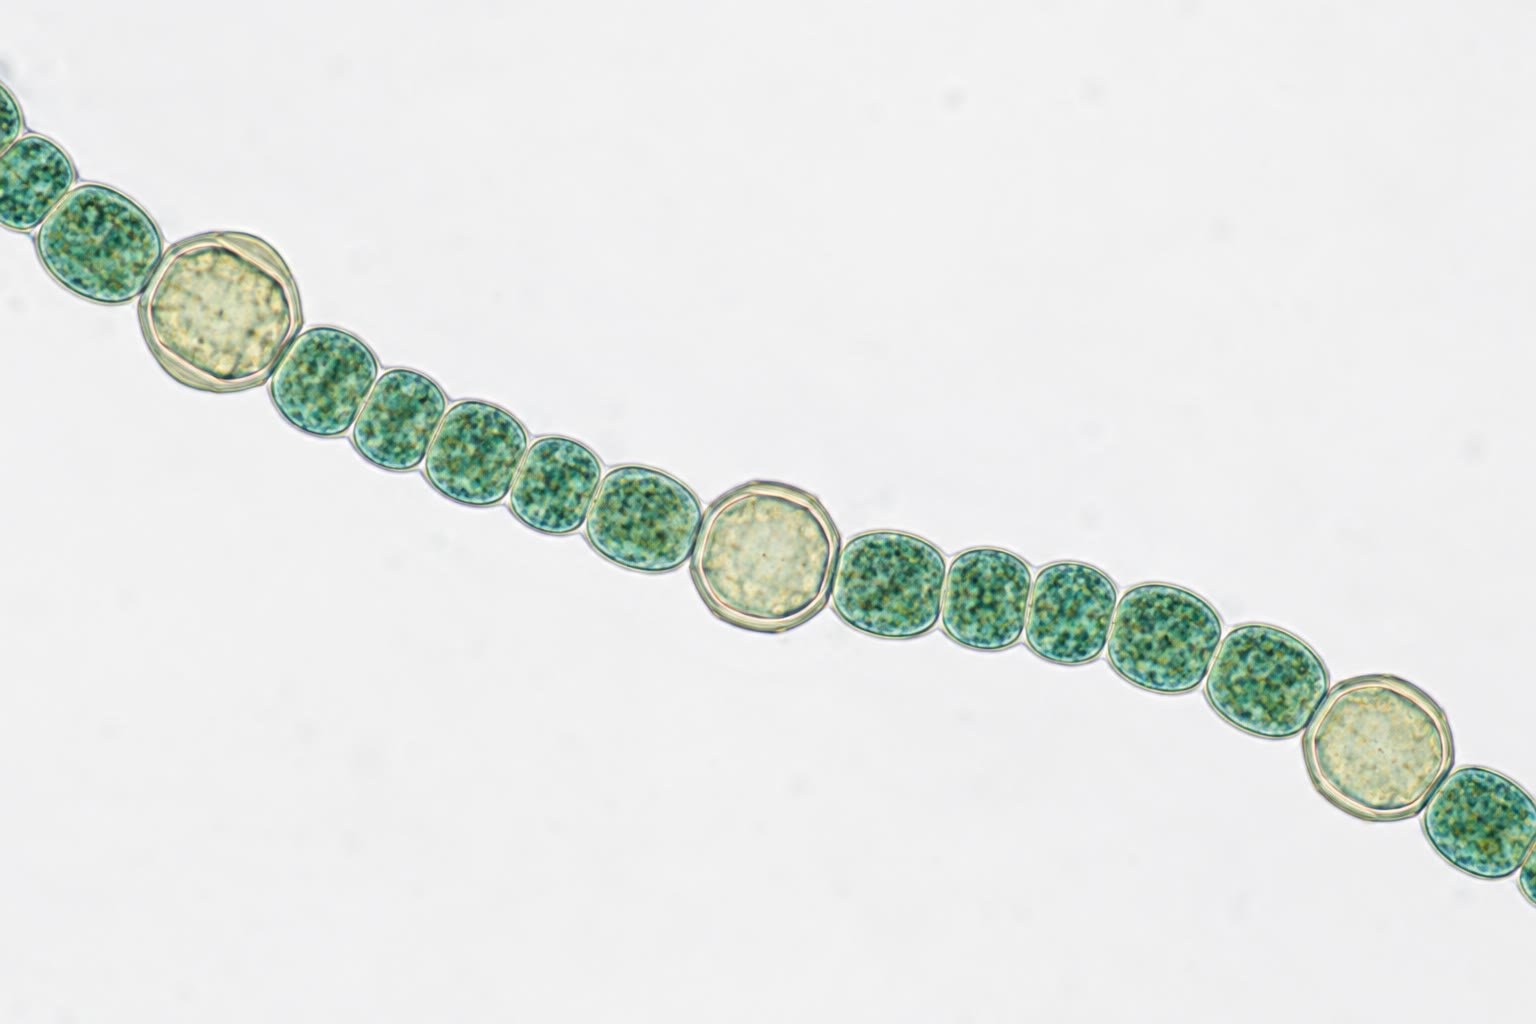
\includegraphics[width=0.62\linewidth]{images/book4/ai/b4-01-anabaena.jpg}

{\small Een draad van \emph{Anabaena}: een keten van groene
fotosynthetische cellen, onderbroken door grotere, blekere heterocysten,
de cellen die stikstof binden.}
\end{omfigure}

\begin{remark}[Rusttoestand]\label{rem:b2:unicellular-diversity:spores}
Sommige grampositieve staafjes (\emph{Bacillus}, \emph{Clostridium})
beantwoorden voedselgebrek met de bouw van een \emph{endospore}: een
kopie van het chromosoom, gewikkeld in verschillende uitgedroogde
mantels, metabool inert en bestand tegen koken, straling en eeuwen
droogte, die ontkiemt wanneer de omstandigheden terugkeren. Veel
\omterm{def:b2:unicellular-diversity:protist}{protisten} doen hetzelfde met een \emph{cyste}. Een rusttoestand is,
naast beweeglijkheid, de andere manier om een slecht seizoen te
overleven.
\end{remark}

\section{Eencellige eukaryoten}

\begin{definition}[Protisten: een graad, geen groep]\label{def:b2:unicellular-diversity:protist}
\emph{Protisten}\index{protist} zijn de eukaryoten die geen dieren,
geen landplanten en geen schimmels zijn --- meestal \omterm{def:b2:unicellular-diversity:unicellular}{eencellig}, sommige
\omterm{def:b2:unicellular-diversity:unicellular}{koloniaal}, enkele (de kelpen) \omterm{def:b2:unicellular-diversity:unicellular}{meercellig}. Ze delen de eukaryote cel
uit het deel van jaar 1 (kern, mitochondriën, endomembranen,
cytoskelet, trilharen met $9+2$-structuur) en verder niets in het
bijzonder: de lijnen waartoe ze behoren, staan even ver van elkaar af
als dieren van planten. Groene algen horen bij de landplanten;
kiezelwieren en bruinwieren vormen een eigen lijn; ciliaten,
dinoflagellaten en de malariaparasiet een andere; amoeben en
slijmzwammen staan dichter bij dieren en schimmels dan bij al deze
groepen. Het woord benoemt een organisatieniveau --- de eukaryote cel
die alleen leeft --- en geen tak van de boom.
\end{definition}

\begin{example}[Vier manieren om als eukaryote cel alleen te leven]\label{ex:b2:unicellular-diversity:four}
\emph{Chlamydomonas}: een eivormige groene alg met een wand van
glycoproteïne zonder cellulose, één bekervormige chloroplast, een
oranje oogvlek die een lichtsensor beschaduwt, zodat de cel tijdens
het draaien weet aan welke kant het licht is, en twee flagellen aan de
voorkant die in een schoolslag slaan; ze is fototroof.
\emph{Paramecium}: een ciliaat, waarvan het hele oppervlak met trilharen
in gecoördineerde golven slaat, met een mondachtige mondgroef die
bacteriën naar voedselvacuolen veegt, twee \omterm{prop:b2:unicellular-diversity:osmoregulation}{contractiele vacuolen} en
twee soorten kernen --- een kleine generatieve \emph{micronucleus} en
een grote werkende \emph{macronucleus} met honderden kopieën van elk
gen; ze is fagotroof. \emph{Amoeba}: geen wand, geen vaste vorm, ze
beweegt en voedt zich met \emph{schijnvoetjes} die door
actinepolymerisatie naar buiten worden geduwd. Het kiezelwier: een
fotosynthetische cel die ingesloten zit in twee overlappende kleppen
van kiezelzuur, als een doos met deksel, zo fijn met poriën versierd
dat men de schalen vroeger gebruikte om microscooplenzen te testen;
bij de deling houdt elke dochtercel één klep en maakt ze een nieuwe,
kleinere klep aan de binnenkant.
\end{example}

\begin{omfigure}
\begin{tikzpicture}[every node/.style={font=\scriptsize}]
  % Paramecium outline (slipper)
  \draw[thick, fill=omProp!8] plot[smooth cycle, tension=0.8] coordinates {(0,0) (1.5,0.9) (3.5,1.1) (5.5,0.7) (6.4,0) (5.5,-0.8) (3.5,-1.1) (1.5,-0.9)};
  % cilia
  \foreach \t in {3,9,...,357} {
    \pgfmathsetmacro{\cx}{3.2+3.25*cos(\t)}
    \pgfmathsetmacro{\cy}{1.08*sin(\t)}
    \pgfmathsetmacro{\dx}{3.2+3.55*cos(\t)}
    \pgfmathsetmacro{\dy}{1.32*sin(\t)}
    \draw[gray] (\cx,\cy) -- (\dx,\dy);
  }
  % macronucleus and micronucleus
  \draw[thick, fill=omDef!40] (3.2,0.05) ellipse (0.9 and 0.45);
  \fill[omDef!90!black] (2.4,0.55) circle (0.13);
  % oral groove and gullet
  \draw[thick, omThm] (4.3,-0.95) .. controls (3.6,-0.5) and (3.3,-0.2) .. (3.0,-0.35);
  \fill[omThm!30] (2.9,-0.45) circle (0.16);
  % food vacuoles
  \foreach \p in {(1.4,-0.3),(1.0,0.35),(4.8,0.35)} \draw[thick, omExo!80!black, fill=omExo!30] \p circle (0.17);
  % contractile vacuoles
  \foreach \c in {(1.2,0.0),(5.2,-0.2)} {
    \draw[thick, omDef] \c circle (0.28);
    \foreach \a in {0,60,...,300} \draw[omDef] \c ++(\a:0.28) -- ++(\a:0.22);
  }
  % labels
  \draw (2.4,0.55) -- (2.7,1.6) node[above] {micronucleus};
  \draw (3.6,0.3) -- (4.8,1.6) node[above] {macronucleus};
  \draw (1.2,0.28) -- (0.3,1.5) node[above, align=center] {contractiele vacuole\\(met straalkanalen)};
  \draw (5.2,-0.48) -- (6.5,-1.5) node[below] {contractiele vacuole};
  \draw (4.3,-0.95) -- (4.7,-1.75) node[below] {mondgroef};
  \draw (2.9,-0.61) -- (2.7,-1.6) node[below, align=center] {celmond en vormende\\voedselvacuole};
  \draw (1.4,-0.47) -- (0.0,-1.5) node[below] {voedselvacuolen};
  \draw (6.35,0.4) -- (6.9,1.2) node[above, align=center] {trilharen};
\end{tikzpicture}

{\small \emph{Paramecium}, schematisch: de bewimperde cortex, de twee
kernen, de mondgroef die naar de celmond leidt waar voedselvacuolen
ontstaan, en de twee stervormige \omterm{prop:b2:unicellular-diversity:osmoregulation}{contractiele vacuolen} die het water
verdrijven dat door osmose binnenkomt.}
\end{omfigure}

\begin{omfigure}
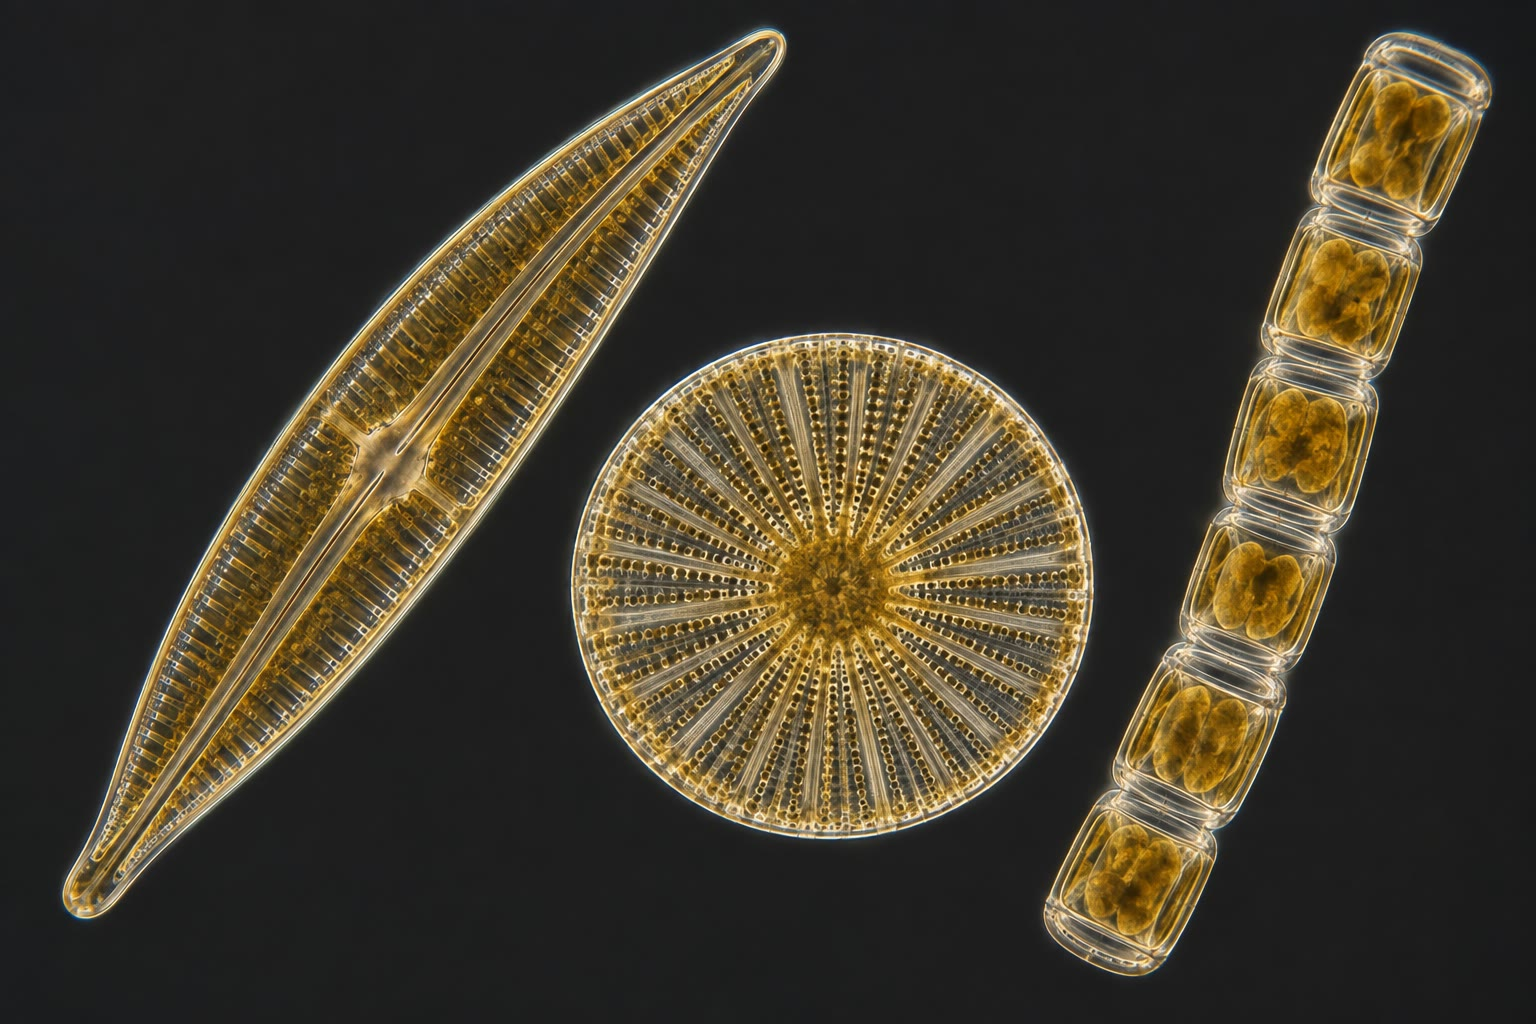
\includegraphics[width=0.6\linewidth]{images/book4/ai/b4-01-diatoms.jpg}

{\small Kiezelwieren in donkerveldmicroscopie: elke cel leeft in een
tweekleppige schaal van kiezelzuur, met een patroon van poriën waardoor
ze met het water uitwisselt.}
\end{omfigure}

\begin{definition}[Voedingswijzen]\label{def:b2:unicellular-diversity:nutrition}
\index{fagotrofie}\index{osmotrofie}\index{mixotrofie}
Een eencellige eukaryoot voedt zich op een van drie manieren, of op
twee tegelijk. \emph{Fototrofie}: hij heeft chloroplasten en maakt zijn
eigen organisch materiaal uit licht en $\mathrm{CO_2}$ (groene algen,
kiezelwieren, dinoflagellaten). \emph{Fagotrofie}: hij omsluit deeltjes
--- bacteriën, andere \omterm{def:b2:unicellular-diversity:protist}{protisten} --- in een voedselvacuole waar
lysosomale enzymen ze verteren (amoeben, ciliaten, kraagflagellaten).
\emph{Osmotrofie}: hij neemt opgeloste moleculen op door zijn membraan,
vaak na enzymen naar buiten te hebben uitgescheiden (gisten, veel
parasieten). \emph{Mixotrofen} zoals \emph{Euglena} bedrijven
fotosynthese in het licht en eten in het donker. Prokaryoten kunnen
niet fagocyteren: de wand verhindert het, en daarom is een \omterm{def:b2:unicellular-diversity:prokaryote}{prokaryoot}
nooit een rover geworden die zijn prooi omsluit.
\end{definition}

\begin{proposition}[Osmoregulatie in zoet water]\label{prop:b2:unicellular-diversity:osmoregulation}
\index{contractiele vacuole}
Een zoetwaterprotist is vanbinnen veel zouter (zo'n \qty{100}{mmol/L}
aan opgeloste stoffen) dan de sloot (ongeveer \qty{1}{mmol/L}), en
zijn membraan laat water door. Water komt dus voortdurend door osmose
binnen, met een snelheid die evenredig is met het oppervlak en met het
verschil in osmotische druk $\Delta\Pi = RT\,\Delta c$ --- ongeveer
\qty{2.4}{bar} voor de bovenstaande waarden. Een cel met een wand
biedt weerstand door turgor; een naakte cel zou binnen enkele minuten
opzwellen en barsten. De \emph{\omterm{prop:b2:unicellular-diversity:osmoregulation}{contractiele vacuole}} is het antwoord:
een reservoir, gevoed door straalkanalen, dat zich vult met water dat
door protongedreven transporters wordt binnengepompt en zich dan
samentrekt en het water via een porie verdrijft, om de paar seconden
tot om de paar minuten. Een \emph{Paramecium} voert elk half uur zijn
eigen volume aan water af; mariene verwanten, in een medium dat even
zout is als zijzelf, hebben helemaal geen \omterm{prop:b2:unicellular-diversity:osmoregulation}{contractiele vacuole}.
\end{proposition}

\section{De fysica van een kleine zwemmer}

\begin{proposition}[Leven bij een laag getal van Reynolds]\label{prop:b2:unicellular-diversity:reynolds}
\index{getal van Reynolds}
Het \emph{\omterm{prop:b2:unicellular-diversity:reynolds}{getal van Reynolds}} $Re = \rho v L/\eta$ vergelijkt
traagheidskrachten met viskeuze krachten voor een lichaam met afmeting
$L$ dat met snelheid $v$ beweegt in een vloeistof met dichtheid $\rho$
en viscositeit $\eta$. Voor een menselijke zwemmer is het ongeveer
$10^6$; voor \emph{Paramecium} (\qty{200}{\micro m}, \qty{1}{mm/s})
is het 0.2, en voor een bacterie $10^{-5}$. Onder
$Re \approx 1$ doet traagheid er niet toe: een cel die ophoudt met
slaan, staat binnen een nanometer stil, water voelt aan als dikke
siroop, en een heen-en-weerbeweging (dezelfde slag voorwaarts en
achterwaarts) levert geen netto verplaatsing op. Kleine zwemmers
gebruiken daarom slagen die niet omkeerbaar zijn: de draaiende schroef
van de bacteriële flagel, de asymmetrische slag van een trilhaar
(stijve krachtslag, gekrulde herstelslag), de schoolslag van
\emph{Chlamydomonas}.
\end{proposition}

\begin{theorem}[De wet van Stokes en bezinken]\label{thm:b2:unicellular-diversity:stokes}
\index{wet van Stokes}
Een bol met straal $r$ en dichtheid $\rho_{\text{cel}}$ die langzaam
door een vloeistof met viscositeit $\eta$ beweegt, ondervindt een
wrijvingskracht $F = 6\pi\eta r v$. Aan zichzelf overgelaten in water met
dichtheid $\rho$ zinkt hij met de eindsnelheid
\[
v_s = \frac{2\,r^2\,(\rho_{\text{cel}} - \rho)\,g}{9\eta},
\]
evenredig met het kwadraat van zijn straal: een cel die tien keer
groter is, zinkt honderd keer sneller. Daarom is het fytoplankton
klein, dragen kiezelwieren stekels en oliedruppels, en zinkt een
\emph{Chlamydomonas} die ophoudt met zwemmen binnen enkele dagen uit
het licht weg.
\end{theorem}
\begin{proof}
Bij de eindsnelheid houdt de wrijving het schijnbare gewicht (gewicht
min opwaartse kracht) in evenwicht: $6\pi\eta r v_s = \tfrac{4}{3}\pi r^3
(\rho_{\text{cel}} - \rho) g$. Oplossen naar $v_s$ geeft de formule.
De wrijvingswet zelf wordt in de natuurkundereeks afgeleid voor
$Re \ll 1$; hier wordt ze als gegeven aangenomen.
\end{proof}

\begin{example}[De val van een kiezelwier]\label{ex:b2:unicellular-diversity:fall}
Een centrisch kiezelwier met straal \qty{10}{\micro m}, \qty{100}{kg/m^3}
dichter dan zeewater ($\eta = \qty{1e-3}{Pa.s}$), zinkt met
$v_s = 2\times 10^{-10}\times 100\times 9.81/(9\times 10^{-3}) =
\qty{2.2e-5}{m/s}$, ongeveer \qty{2}{m} per dag: het zou de verlichte
laag van \qty{50}{m} in minder dan een maand verlaten. Zijn populaties
overleven doordat turbulentie het water omroert, doordat oliedruppels en
een lage dichtheid $\rho_{\text{cel}} - \rho$ verkleinen, en doordat een
cel die onderweg zinkt en zich deelt nakomelingen achterlaat die weer
omhoog worden gevoerd.
\end{example}

\begin{omfigure}
\begin{tikzpicture}
\begin{axis}[
  width=0.8\linewidth, height=6.0cm,
  axis x line=bottom, axis y line=left,
  xmode=log, ymode=log,
  xmin=0.5, xmax=200, ymin=1e-3, ymax=1e4,
  xlabel={straal (\unit{\micro m})}, ylabel={zinksnelheid (\unit{\micro m/s})},
  xlabel style={font=\small, at={(axis description cs:0.5,-0.1)}, anchor=north},
  ylabel style={font=\small},
  tick label style={font=\small},
  clip=false,
]
\addplot[very thick, omDef, domain=0.5:200, samples=40] {0.218*x^2};
\addplot[only marks, mark=*, mark size=1.8pt, omThm] coordinates {(1,0.218) (10,21.8) (100,2180)};
\node[font=\scriptsize, anchor=west] at (axis cs:1.15,0.218) {bacterie};
\node[font=\scriptsize, anchor=west] at (axis cs:11.5,21.8) {kiezelwier};
\node[font=\scriptsize, anchor=east] at (axis cs:85,2180) {grote protist};
\end{axis}
\end{tikzpicture}

{\small Zinksnelheid volgens Stokes als functie van de straal voor cellen die
\qty{100}{kg/m^3} dichter zijn dan water. De helling 2 op logaritmische
assen is de $r^2$-wet: een bacterie zinkt een centimeter per dag, een grote
\omterm{def:b2:unicellular-diversity:protist}{protist} een paar meter per uur.}
\end{omfigure}

\section{Voortplanting en seks in één cel}

\begin{definition}[Wijzen van deling]\label{def:b2:unicellular-diversity:division}
\index{binaire deling}\index{knopvorming}\index{meervoudige deling}
Een \omterm{def:b2:unicellular-diversity:unicellular}{eencellig organisme} plant zich voort door zich te delen. \emph{Binaire
deling}: de cel groeit tot tweemaal haar grootte en splitst zich in twee
gelijke dochtercellen (bacteriën, \emph{Paramecium}, \emph{Amoeba}).
\emph{Knopvorming}: een kleine dochtercel groeit uit de moedercel en laat
los (gist; de moedercel houdt een litteken over en kan zo'n twintig keer
knoppen). \emph{Meervoudige deling}: de cel groeit sterk en deelt zich
dan binnen de moederwand enkele malen snel na elkaar, waarna ze 4, 8,
16 of meer dochtercellen tegelijk vrijlaat (\emph{Chlamydomonas}, de
malariaparasiet in een rode bloedcel). Onder constante omstandigheden
groeit het aantal cellen exponentieel, $N(t) = N_0\,2^{t/T}$, met $T$ de
\emph{generatietijd}\index{generatietijd}: twintig minuten voor
\emph{E.~coli} in een rijk medium, een dag voor veel algen, een week voor
sommige ciliaten. (Groei als functie van het voedsel komt aan bod in
\cref{ch:b2:microbial-metabolism}.)
\end{definition}

\begin{proposition}[Seks zonder voortplanting: conjugatie bij \emph{Paramecium}]\label{prop:b2:unicellular-diversity:conjugation}
\index{conjugatie!ciliaten}
Twee exemplaren van \emph{Paramecium} van complementaire paringstypen
hechten zich met hun mondzijde aan elkaar. In elk ervan ondergaat de
diploïde micronucleus meiose tot vier haploïde kernen, waarvan er drie
degenereren; de overlevende deelt zich door mitose in een stationaire
en een migrerende kern, en de twee cellen wisselen hun migrerende kernen
uit over de verbinding. Elke cel versmelt dan haar stationaire kern met
de ontvangen kern, en de twee partners gaan uiteen, elk met een nieuwe
diploïde micronucleus met hetzelfde genotype als die van de partner. De
oude macronucleus valt uiteen en uit de nieuwe micronucleus wordt een
nieuwe opgebouwd. Er is geen nieuwe cel gemaakt: conjugatie is
genetische menging --- meiose en bevruchting,
\cref{ch:b2:meiosis-heredity} --- losgekoppeld van vermenigvuldiging.
Bacteriële conjugatie, die een \omterm{def:b2:unicellular-diversity:prokaryote}{plasmide} in één richting van donor naar
ontvanger overdraagt, is een ander proces met dezelfde naam
(\cref{ch:b2:genome-diversification}).
\end{proposition}

\begin{omfigure}
\begin{tikzpicture}[every node/.style={font=\scriptsize}]
  \foreach \i/\x in {0/0,1/3.6,2/7.2,3/10.8} {
    \draw[thick, fill=omProp!8] (\x,0.55) ellipse (1.0 and 0.5);
    \draw[thick, fill=omProp!8] (\x,-0.55) ellipse (1.0 and 0.5);
  }
  % stage 0: two cells, diploid micronuclei 2n
  \fill[omDef!90!black] (0,0.55) circle (0.12); \node[right] at (0.15,0.55) {$2n$};
  \fill[omDef!90!black] (0,-0.55) circle (0.12); \node[right] at (0.15,-0.55) {$2n$};
  \node[below, align=center] at (0,-1.15) {twee cellen hechten};
  % stage 1: meiosis, 4 haploid, 3 degenerate
  \foreach \dy in {0.55,-0.55} {
    \fill[omDef!90!black] (3.6-0.3,\dy+0.15) circle (0.08);
    \fill[gray!60] (3.6+0.1,\dy+0.2) circle (0.06);
    \fill[gray!60] (3.6+0.3,\dy-0.05) circle (0.06);
    \fill[gray!60] (3.6-0.1,\dy-0.25) circle (0.06);
  }
  \node[below, align=center] at (3.6,-1.15) {meiose:\\4 haploïde kernen,\\drie degenereren};
  % stage 2: mitosis, exchange
  \foreach \dy in {0.55,-0.55} {
    \fill[omDef!90!black] (7.2-0.35,\dy) circle (0.08);
    \fill[omThm] (7.2+0.35,\dy) circle (0.08);
  }
  \draw[->, thick, omThm] (7.55,0.45) -- (7.55,-0.45);
  \draw[->, thick, omThm] (6.85,-0.45) -- (6.85,0.45);
  \node[below, align=center] at (7.2,-1.15) {mitose; migrerende\\kernen (rood)\\worden uitgewisseld};
  % stage 3: fusion 2n
  \fill[omDef!90!black] (10.8,0.55) circle (0.12); \node[right] at (10.95,0.55) {$2n$};
  \fill[omDef!90!black] (10.8,-0.55) circle (0.12); \node[right] at (10.95,-0.55) {$2n$};
  \node[below, align=center] at (10.8,-1.15) {bevruchting:\\nieuwe identieke diploïde\\kernen; cellen gaan uiteen};
  \foreach \x in {1.3,4.9,8.5} \draw[->, thick, gray] (\x,0) -- (\x+1.0,0);
\end{tikzpicture}

{\small Conjugatie bij \emph{Paramecium}. Twee cellen wisselen haploïde
kernen uit en gaan uiteen, elk met een gerecombineerde diploïde
micronucleus; het aantal cellen is niet veranderd.}
\end{omfigure}

\section{Op weg naar meercelligheid}

\begin{proposition}[De volvocale reeks]\label{prop:b2:unicellular-diversity:volvox}
\index{Volvox@\emph{Volvox}}\index{meercelligheid, oorsprong van}
Bij de groene algen toont één lijn, in levende soorten, de stappen van
één cel naar een lichaam. \emph{Chlamydomonas} leeft alleen.
\emph{Gonium} is een platte plaat van 4 tot 16 identieke cellen die samen
zwemmen. \emph{Pandorina} en \emph{Eudorina} zijn holle bollen van 16
tot 32 cellen, nog allemaal gelijk, elk in staat een nieuwe kolonie te
stichten. \emph{Pleodorina} heeft enkele kleine cellen die alleen
zwemmen en zich nooit delen. \emph{Volvox} is een bol van \num{500} tot
\num{50000} kleine, geflagelleerde somatische cellen, die met de kolonie
zullen sterven, rond een handvol grote kiemcellen (gonidia) die zich
delen tot dochterbollen binnen de moeder. Somatische en kiemcellen zijn
verschenen: dit is de drempel van de meercelligheid, in deze lijn
overschreden zo'n \num{200} miljoen jaar geleden en, onafhankelijk
daarvan, minstens vijfentwintig keer elders in de levensboom --- bij
dieren, planten, schimmels, bruinwieren, roodwieren en verscheidene
bacteriegroepen.
\end{proposition}
\begin{proof}[Bewijsmateriaal]
De moleculaire fylogenie van de volvocale algen, opgebouwd uit tientallen
genen, plaatst \emph{Chlamydomonas} aan de basis en \emph{Volvox}
aan de toppen, met de koloniale vormen ertussen en een aantal cellen
dat langs de takken toeneemt; het genoom van \emph{Volvox carteri}
(2010) verschilt van dat van \emph{Chlamydomonas} in enkele honderden
genen, vooral die van de extracellulaire matrix die de cellen bijeenhoudt
en van de regulatoren die de deling in somatische cellen stilleggen. De
overgang vergde opmerkelijk weinig nieuw genetisch materiaal.
\end{proof}

\begin{omfigure}
\begin{tikzpicture}[every node/.style={font=\scriptsize}]
  % Chlamydomonas
  \draw[thick, fill=omProp!25] (0,0) circle (0.22);
  \node[below=0.35cm, align=center] at (0,0) {\emph{Chlamydomonas}\\1 cel};
  % Gonium plate
  \begin{scope}[xshift=2.2cm]
    \foreach \x in {-0.3,0,0.3} \foreach \y in {-0.3,0,0.3} \draw[thick, fill=omProp!25] (\x,\y) circle (0.14);
    \draw[gray, dashed] (-0.55,-0.55) rectangle (0.55,0.55);
    \node[below=0.7cm, align=center] at (0,0) {\emph{Gonium}\\plaat van 8--16};
  \end{scope}
  % Eudorina ball
  \begin{scope}[xshift=4.5cm]
    \draw[gray, dashed] (0,0) circle (0.6);
    \foreach \a in {0,45,...,315} \draw[thick, fill=omProp!25] (\a:0.55) circle (0.13);
    \draw[thick, fill=omProp!25] (0,0.1) circle (0.13);
    \node[below=0.7cm, align=center] at (0,0) {\emph{Eudorina}\\bol van 32,\\allemaal gelijk};
  \end{scope}
  % Pleodorina
  \begin{scope}[xshift=7.4cm]
    \draw[gray, dashed] (0,0) circle (0.7);
    \foreach \a in {0,30,...,330} \draw[thick, fill=omProp!25] (\a:0.62) circle (0.09);
    \foreach \a in {60,180,300} \draw[thick, fill=omProp!60] (\a:0.62) circle (0.14);
    \node[below=0.8cm, align=center] at (0,0) {\emph{Pleodorina}\\sommige cellen\\zwemmen alleen};
  \end{scope}
  % Volvox
  \begin{scope}[xshift=10.6cm]
    \draw[thick, fill=omProp!6] (0,0) circle (0.95);
    \foreach \a in {0,12,...,348} \fill[omProp!70] (\a:0.9) circle (0.035);
    \foreach \a in {0,12,...,348} \fill[omProp!50] (\a:0.72) circle (0.03);
    \foreach \p in {(0.25,0.2),(-0.3,-0.25),(0.1,-0.4),(-0.2,0.35)} \draw[thick, omThm, fill=omThm!40] \p circle (0.13);
    \node[below=1.05cm, align=center] at (0,0) {\emph{Volvox}\\duizenden somatische cellen\\en enkele kiemcellen (rood)};
  \end{scope}
  \foreach \x in {0.5,3.0,5.3,8.3} \draw[->, gray] (\x,0) -- (\x+0.6,0);
\end{tikzpicture}

{\small De volvocale reeks: één cel, een plaat, een holle bol van
identieke cellen, een bol waarin sommige cellen de deling hebben
opgegeven, en \emph{Volvox}, waar duizenden sterfelijke somatische cellen
enkele kiemcellen omringen.}
\end{omfigure}

\begin{omfigure}
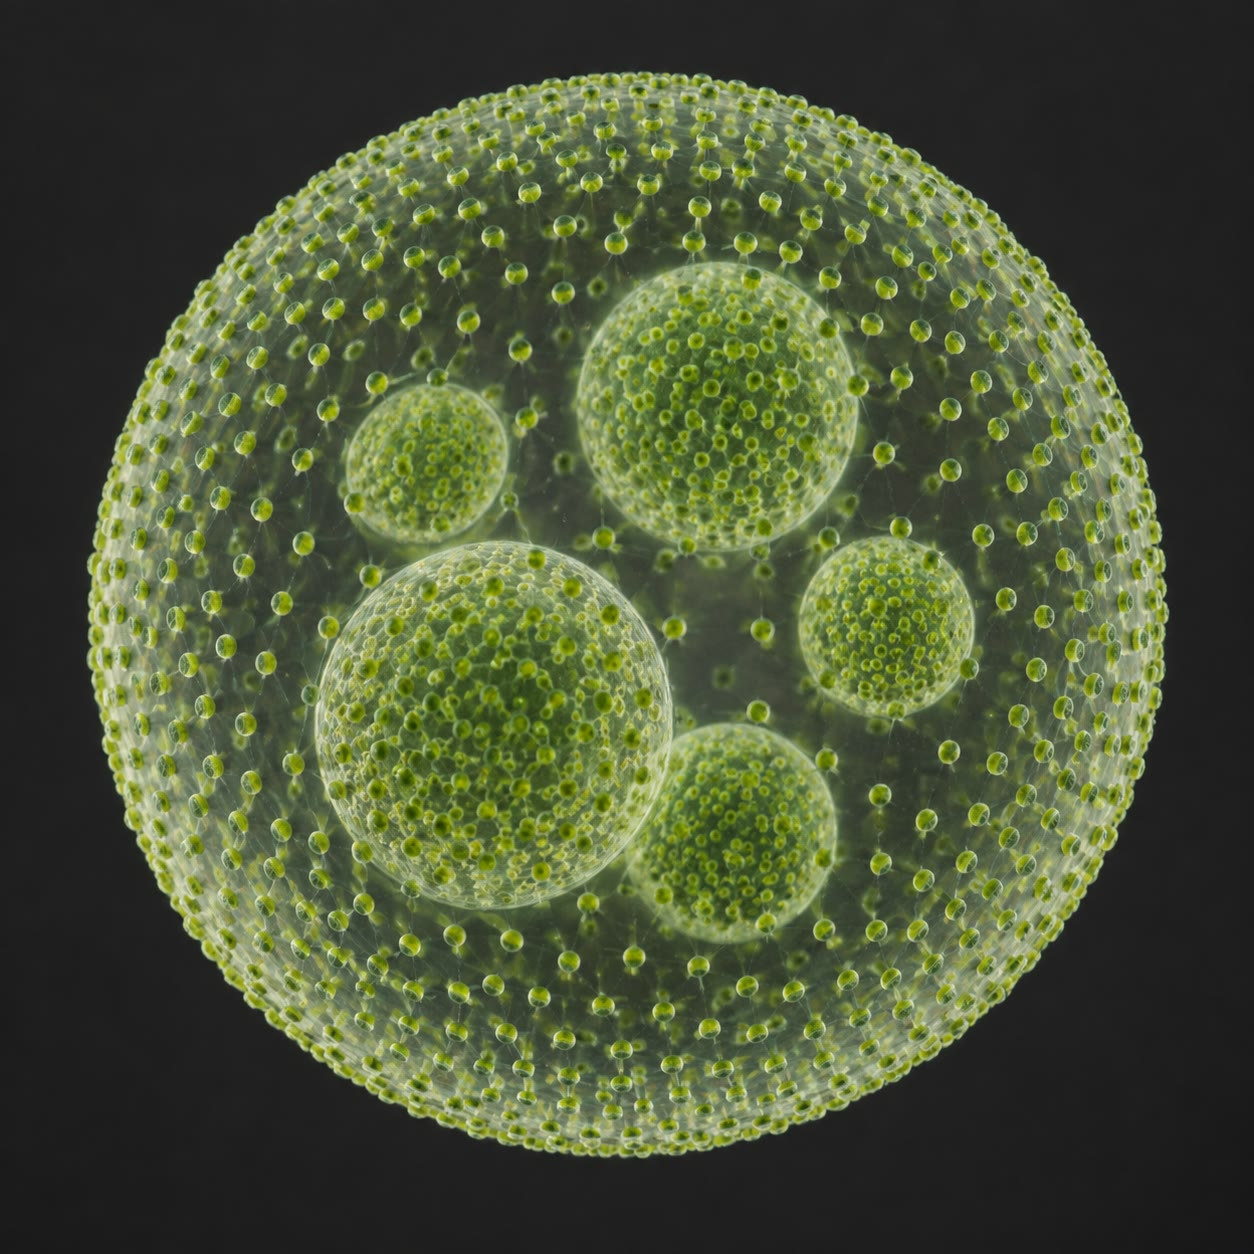
\includegraphics[width=0.55\linewidth]{images/book4/ai/b4-01-volvox.jpg}

{\small Een kolonie van \emph{Volvox}: een holle groene bol van
geflagelleerde cellen, met dochterkolonies die erbinnen groeien.}
\end{omfigure}

\begin{remark}[Waarom de arbeid verdelen?]\label{rem:b2:unicellular-diversity:whydivide}
Bij deze algen kan een cel niet tegelijk zwemmen en zich delen: de
basale lichaampjes die de flagellen verankeren, zijn nodig om de
spoelfiguur te organiseren. Een enkele cel wisselt beide af; een kleine
kolonie kan het zich permitteren te stoppen met zwemmen terwijl al haar
cellen zich delen; een grote kolonie zou tijdens de uren die haar deling
kost uit het licht wegzinken (de \omterm{thm:b2:unicellular-diversity:stokes}{wet van Stokes},
\cref{thm:b2:unicellular-diversity:stokes}). Voorbij een zekere grootte
loont het om sommige cellen te laten zwemmen terwijl andere zich delen,
ook al gaan hun nakomelingen verloren --- en zo ontstaat een soma. De
kraagflagellaten, geflagelleerde cellen met een kraag, waarvan de cel
een kopie is van de voedingscel van een spons, tonen dezelfde eerste
stappen op de tak die naar de dieren leidde.
\end{remark}

\section{Opgaven}

\begin{exercise}[$\star$]\label{exo:b2:unicellular-diversity:1}
Definieer \omterm{def:b2:unicellular-diversity:unicellular}{eencellig}, \omterm{def:b2:unicellular-diversity:unicellular}{koloniaal} en \omterm{def:b2:unicellular-diversity:unicellular}{meercellig}, en deel \emph{E.~coli},
\emph{Gonium}, \emph{Volvox} en een gistcel met een reden in de juiste
categorie in.
\end{exercise}

\begin{exercise}[$\star$]\label{exo:b2:unicellular-diversity:2}
Bereken de \omterm{prop:b2:unicellular-diversity:surface}{oppervlakte-volumeverhouding} van een coccus met straal
\qty{0.5}{\micro m} en van een bolvormige \omterm{def:b2:unicellular-diversity:protist}{protist} met straal
\qty{50}{\micro m}. Welke van de twee ademt sneller per eenheid
cytoplasma, en waarom?
\end{exercise}

\begin{exercise}[$\star$]\label{exo:b2:unicellular-diversity:3}
Geef drie structurele verschillen tussen een bacterie en een eencellige
eukaryoot, en één ding dat een amoebe wel kan en een bacterie niet.
\end{exercise}

\begin{exercise}[$\star$]\label{exo:b2:unicellular-diversity:4}
Geef de functie van elk van de volgende structuren van
\emph{Paramecium}: trilharen, mondgroef, voedselvacuole, \omterm{prop:b2:unicellular-diversity:osmoregulation}{contractiele
vacuole}, macronucleus, micronucleus.
\end{exercise}

\begin{exercise}[$\star\star$]\label{exo:b2:unicellular-diversity:5}
Hoelang doet diffusie er, met $D = \qty{5e-10}{m^2/s}$ voor een
metaboliet in het cytoplasma, over om een bacterie van \qty{1}{\micro m}
en een amoebe van \qty{500}{\micro m} over te steken? Licht toe wat de
amoebe moet doen en de bacterie niet.
\end{exercise}

\begin{exercise}[$\star\star$]\label{exo:b2:unicellular-diversity:6}
Bereken het \omterm{prop:b2:unicellular-diversity:reynolds}{getal van Reynolds} van een \emph{Paramecium} (\qty{200}{\micro
m}, \qty{1}{mm/s}), van een bacterie (\qty{2}{\micro m}, \qty{20}{\micro
m/s}) en van een menselijke zwemmer (\qty{2}{m}, \qty{1}{m/s}), met
$\rho = \qty{1000}{kg/m^3}$ en $\eta = \qty{1e-3}{Pa.s}$. Waarom kan een
zwemmer na een slag doorglijden en een bacterie niet?
\end{exercise}

\begin{exercise}[$\star\star$]\label{exo:b2:unicellular-diversity:7}
Een kiezelwier met straal \qty{10}{\micro m} is \qty{100}{kg/m^3}
dichter dan water. Bereken zijn zinksnelheid en de tijd om
\qty{50}{m} te zakken. Met welke factor verandert die tijd als de cel
haar straal halveert? En als ze haar dichtheidsoverschot tot
\qty{20}{kg/m^3} terugbrengt?
\end{exercise}

\begin{exercise}[$\star\star$]\label{exo:b2:unicellular-diversity:8}
Beschouw een \emph{Paramecium} als een ellipsoïde met halve assen \num{100},
\num{25} en \qty{25}{\micro m} ($V = \tfrac{4}{3}\pi abc$). Hij verdrijft
elke \qty{30}{min} zijn eigen volume aan water. Bereken de waterinstroom
in \unit{\micro m^3/s} en in liter per seconde.
\end{exercise}

\begin{exercise}[$\star\star$]\label{exo:b2:unicellular-diversity:9}
Een lokstof verdubbelt in concentratie over \qty{1}{mm}. Wat is het
relatieve verschil tussen de twee uiteinden van een bacterie van
\qty{1}{\micro m}? En tussen het begin en het einde van een run van
\qty{1}{s} bij \qty{20}{\micro m/s}? Het tellen van $N$ moleculen heeft
een relatieve fout van ongeveer $1/\sqrt{N}$: leg uit waarom de bacterie
tijdstippen vergelijkt in plaats van zijden.
\end{exercise}

\begin{exercise}[$\star\star\star$]\label{exo:b2:unicellular-diversity:10}
\emph{Thiomargarita namibiensis} is een bolvormige zwavelbacterie met
een diameter van \qty{500}{\micro m}, waarvan het cytoplasma een schil
van \qty{2}{\micro m} dik vormt rond een vacuole met nitraat. Bereken de
verhouding van haar oppervlak tot haar \emph{cytoplasmatische} volume en
vergelijk met \emph{E.~coli} (een cilinder met straal \qty{0.5}{\micro m};
verwaarloos de uiteinden). Leg uit hoe de vacuole haar zo groot laat
worden, en waarvoor het nitraat dient.
\end{exercise}

\begin{exercise}[$\star\star\star$]\label{exo:b2:unicellular-diversity:11}
Bij \emph{Volvox} delen de somatische cellen zich nooit en sterven ze met
de kolonie. Leg met behulp van de beperking door de flagellen en de \omterm{thm:b2:unicellular-diversity:stokes}{wet
van Stokes} uit waarom zulke cellen de moeite waard zijn in een kolonie
van \num{10000} cellen maar niet in een van 16, en waarom de kiemcellen
de grootste cellen van de bol zijn.
\end{exercise}

\begin{exercise}[$\star\star\star$]\label{exo:b2:unicellular-diversity:12}
``\omterm{def:b2:unicellular-diversity:protist}{Protist} is een graad, geen clade.'' Licht het onderscheid toe aan de
hand van de lijnen die in dit hoofdstuk zijn genoemd, en zeg waarom
dezelfde uitspraak klopt voor ``\omterm{def:b2:unicellular-diversity:prokaryote}{prokaryoot}'' en niet voor ``cyanobacterie''.
\end{exercise}

\section{Vraagstuk: een druppel slootwater}

\begin{problem}[{Weekendvraagstuk --- een monster slootwater wordt geteld,
opgekweekt en onderzocht op de fysica die zijn cellen beheerst, met als
besluit de water- en energiebalans van een groene alg}]
\label{pb:b2:unicellular-diversity:1}
Een vijver van \qty{1000}{m^3} wordt in het voorjaar bemonsterd. Onder de
microscoop toont een telkamer, waarvan het raster \qty{1}{mm}$\times$\qty{1}{mm}
beslaat onder een dekglaasje dat \qty{0.1}{mm} erboven wordt gehouden,
24 cellen van \emph{Chlamydomonas} (bollen met straal \qty{5}{\micro m},
dichtheid \qty{1050}{kg/m^3}). Neem $\rho = \qty{1000}{kg/m^3}$,
$\eta = \qty{1e-3}{Pa.s}$, $g = \qty{9.81}{m/s^2}$, $R =
\qty{8.314}{J/mol/K}$, $T = \qty{293}{K}$, $D = \qty{1.9e-9}{m^2/s}$
voor $\mathrm{CO_2}$ in water.

\medskip
\noindent\textbf{Deel I --- Tellen.}
\begin{enumerate}
  \item Bereken het volume water onder het raster, in microliter.
  \item Leid de dichtheid van \emph{Chlamydomonas} in de vijver af, in
        cellen per milliliter.
  \item Bereken het volume en de \omterm{prop:b2:unicellular-diversity:surface}{oppervlakte-volumeverhouding} van één
        cel.
  \item Welk deel van het volume van het vijverwater nemen deze cellen
        in?
  \item Hoeveel exemplaren van \emph{Chlamydomonas} bevat de vijver?
  \item Er is ook een draadvormige cyanobacterie aanwezig. Geef twee
        kenmerken, zichtbaar onder de microscoop, die haar van de alg
        onderscheiden.
\end{enumerate}

\medskip
\noindent\textbf{Deel II --- Groei.}
Het monster wordt in het licht bewaard en na \qty{48}{h} opnieuw geteld:
\num{384} cellen onder het raster.
\begin{enumerate}[resume]
  \item Bereken de \omterm{def:b2:unicellular-diversity:division}{generatietijd} $T$.
  \item Bereken de groeisnelheidsconstante $k$ in $N = N_0 e^{kt}$, in
        \unit{h^{-1}}.
  \item Hoelang zou de vijverpopulatie er bij dit tempo over doen om
        \qty{1e8}{} cellen per milliliter te bereiken?
  \item Geef drie redenen waarom dat niet zal gebeuren.
  \item Als de cellen alleen groeien tijdens de \qty{12}{h} daglicht en
        's nachts helemaal niet, hoelang duurt dezelfde toename dan?
  \item \emph{Chlamydomonas} deelt zich door \omterm{def:b2:unicellular-diversity:division}{meervoudige deling} en laat
        4, 8 of 16 dochtercellen tegelijk vrij. Leg uit waarom een
        \omterm{def:b2:unicellular-diversity:division}{generatietijd} toch goed door de telling wordt bepaald.
\end{enumerate}

\medskip
\noindent\textbf{Deel III --- De fysica van de cel.}
\begin{enumerate}[resume]
  \item Bereken het \omterm{prop:b2:unicellular-diversity:reynolds}{getal van Reynolds} van een cel die met
        \qty{100}{\micro m/s} zwemt.
  \item Een cel met massa $m$ die ophoudt met het slaan van haar
        flagellen, glijdt een afstand $mv/(6\pi\eta r)$ door. Bereken die.
  \item Bereken de zinksnelheid van een cel die is gestopt met
        zwemmen.
  \item Vergelijk de tijd om \qty{1}{m} te zinken met de tijd om
        \qty{1}{m} omhoog te zwemmen.
  \item De vijver bevat \qty{10}{\micro mol/L} opgelost
        $\mathrm{CO_2}$. Bereken de maximale diffusieve aanvoer van
        $\mathrm{CO_2}$ naar een cel, in moleculen per seconde.
  \item Een cel bevat \qty{100}{pg} koolstof en verdubbelt die in
        één generatie. Bereken haar gemiddelde koolstofvraag in moleculen
        per seconde, en de verhouding van aanvoer tot vraag.
  \item Herhaal de vergelijking voor een hypothetische cel met straal
        \qty{50}{\micro m} en dezelfde koolstofdichtheid. Trek een conclusie.
\end{enumerate}

\medskip
\noindent\textbf{Deel IV --- Water en energie.}
Het cytoplasma bevat \qty{100}{mmol/L} opgeloste stoffen, de vijver
\qty{1}{mmol/L}. De hydraulische geleidbaarheid van het membraan is $L_p =
\qty{1e-14}{m.s^{-1}.Pa^{-1}}$ (volumeflux van water per eenheid
oppervlak per eenheid drukverschil). De hydrolyse van één ATP levert
\qty{50}{kJ/mol} op; de fixatie van één koolstofatoom kost drie ATP.
\begin{enumerate}[resume]
  \item Bereken het verschil in osmotische druk over het membraan.
  \item Bereken het volume water dat per seconde de cel binnenkomt, in
        \unit{\micro m^3/s}.
  \item Hoelang zou de cel er zonder \omterm{prop:b2:unicellular-diversity:osmoregulation}{contractiele vacuole} over doen om
        haar volume te verdubbelen?
  \item Bereken het minimale vermogen dat nodig is om dit water tegen
        de osmotische druk in naar buiten te werken.
  \item Reken het om naar ATP-moleculen per seconde en vergelijk met de
        ATP die de cel aan koolstoffixatie besteedt (vraag 18).
  \item Formuleer het resultaat: de waterinstroom van de cel, de tijd
        waarin ze zou barsten, en het deel van haar energie dat het
        droog houden kost.
\end{enumerate}
\end{problem}
